\section{\textsc{CrossSteer}: Does a Source Direction Transfer?}
\label{sec:crosssteer}

We test whether a correct-minus-incorrect source direction improves a target
model under the frozen protocol in Section~\ref{sec:crosssteer-no-leakage}.
The source direction comes from
\textsc{Qwen2.5-Math}-1.5B-Instruct trajectories (GSM8K IDs 0--99).  The
target is \textsc{Qwen2.5}-1.5B-Instruct, the aligned-orientation boundary
case from the submitted version; \textsc{R1-Distill}, the historical
opposite-orientation repair target, fails its frozen readiness gate under its
model-valid decoder (below).  Selection uses IDs 100--199; the locked test
uses IDs 200--299.  All
methods share the target, greedy decoder, \texttt{decode\_last}
hook, RMS perturbation budget, and problem-indexed baseline, and have the same online form: one RMS-normalized residual-stream vector addition per generated token.  We compare
\textsc{CrossSteer} with target calibration, CAA, ActAdd, SAE sparse activation,
coordinate-sparse CAA, sign reversal, matched random, and no steering; their
offline supervision and online cost are detailed in Appendix~\ref{app:repro} (Table~\ref{tab:steering-budget}).

Selection is allowed only after provenance, EOS, hash, and baseline-parity checks.
Eligible cells must keep the repeated-four-gram increase below $0.05$ and mean
length below $1.5\times$ baseline; validation then selects accuracy with
deterministic ties.  Locked reports include paired uncertainty, repairs/breaks,
length, repetition, truncation, and stop reasons.

We evaluated the R1-Distill target separately with its model-valid 32,768-token sampled
decoder.  Its readiness set contained severe repetition in two outputs
(10\%; 2/20), above the preregistered 5\% ceiling, so we stopped that branch before calibration or intervention.

\subsection{Source transfer versus target labels}

We compare source transfer with target-local supervision at budgets
$0,5,10,20,50,100$.  Budget 0 uses the source vector; nonzero budgets are nested,
hash-selected, class-stratified target subsets.  Layer, strength, decoder, and
locked examples remain fixed.

\begin{table}[tbp]
\centering
\scriptsize
\setlength{\tabcolsep}{2.5pt}
\caption{Frozen target-label-budget curve on GSM8K IDs 200--299.  All rows
use the target-calibrated layer, strength and decoder; label budget 0 uses the
external source vector.  Intervals/tests are paired against the shared 62\%
baseline, with Holm correction over all six rows.}
\label{tab:label-efficiency}
\begin{tabular}{@{}rrrrr@{}}
\toprule
Labels & Acc. & $\Delta$ pp [95\% CI] & R/B & $p_{\mathrm{Holm}}$ \\
\midrule
0 & 0.68 & $+6$ [$-1,+13$] & 9/3 & 0.7300 \\
5 & 0.73 & $+11$ [$+4,+18$] & 13/2 & \textbf{0.0443} \\
10 & 0.64 & $+2$ [$-6,+10$] & 10/8 & 1.0000 \\
20 & 0.63 & $+1$ [$-7,+9$] & 9/8 & 1.0000 \\
50 & 0.67 & $+5$ [$-4,+14$] & 12/7 & 1.0000 \\
100 & 0.65 & $+3$ [$-6,+12$] & 12/9 & 1.0000 \\
\bottomrule
\end{tabular}
\end{table}

\paragraph{Result.}
Table~\ref{tab:label-efficiency} reports the frozen label-budget
curve.  Five target labels give the only corrected positive row: 73\% versus 62\%
baseline ($+11$~pp, 95\% CI $[+4,+18]$, Holm-adjusted $p=0.0443$).  The
zero-label source row is inconclusive (68\%, $+6$~pp, CI $[-1,+13]$), and the
10--100-label rows are non-monotone and non-significant.  The five-label
subset is the single hash-selected, class-stratified subset fixed before
evaluation (calibration indices 6, 39, 66, 73, 80 of target-calibration IDs
100--199); the adjacent 10-label row ($+2$~pp) and the absence
of dose--response indicate that this cell is not a general label-efficiency
effect.  Budget 0 uses the target-calibrated layer and strength, while the
locked family uses
\textsc{CrossSteer}'s own validation-selected values, hence 0.68 vs.\ 0.61.

\subsection{Locked in-domain comparison}
\label{sec:crosssteer-results}

Each eligible method is run once on locked GSM8K IDs 200--299 against a
byte-verified shared baseline, so every delta is problem-paired.

\begin{table*}[tbp]
\centering
\scriptsize
\setlength{\tabcolsep}{4pt}
\caption{Locked Qwen-Instruct GSM8K comparison.  Every row uses the same
baseline and passed the behavior guard; the maximum truncation rate is 6\%.}
\label{tab:crosssteer-locked}
\begin{tabular}{@{}lrrrrrrr@{}}
\toprule
Method & $\ell$ & $\alpha$ & Base acc. & Steered acc. & $\Delta$ pp (95\% CI) & R/B & $p_{\mathrm{Holm}}$ \\
\midrule
ActAdd & 20 & 0.05 & 0.620 & 0.630 & +1.0 [-5.0, +7.0] & 6/5 & 1.0000 \\
CAA & 20 & 0.1 & 0.620 & 0.700 & +8.0 [+0.0, +16.0] & 13/5 & 0.7383 \\
\textsc{CrossSteer} & 14 & 0.025 & 0.620 & 0.610 & -1.0 [-6.0, +4.0] & 3/4 & 1.0000 \\
Matched random & 24 & 0.025 & 0.620 & 0.630 & +1.0 [-2.0, +4.0] & 2/1 & 1.0000 \\
Sign-reversed & 24 & 0.1 & 0.620 & 0.680 & +6.0 [-1.0, +13.0] & 10/4 & 1.0000 \\
SAE sparse & 20 & 0.1 & 0.620 & 0.690 & +7.0 [+0.0, +14.0] & 10/3 & 0.7383 \\
Sparse CAA & 20 & 0.2 & 0.620 & 0.650 & +3.0 [-5.0, +12.0] & 11/8 & 1.0000 \\
Target-calibrated & 20 & 0.1 & 0.620 & 0.650 & +3.0 [-6.0, +12.0] & 12/9 & 1.0000 \\
\bottomrule
\end{tabular}
\end{table*}

\begin{figure*}[tbp]
\centering
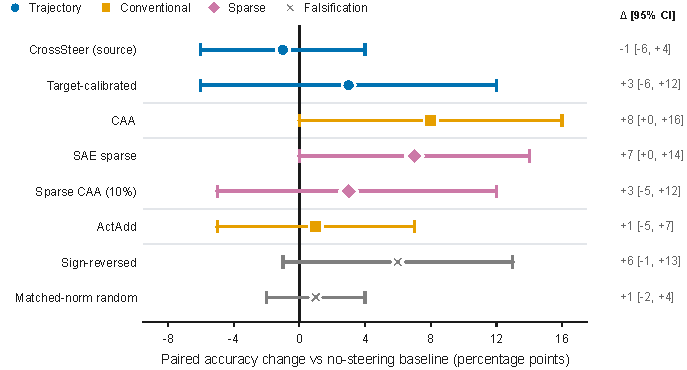
\includegraphics[width=0.88\linewidth]{figures/fig_locked_comparison_forest.pdf}
\caption{Locked GSM8K paired changes from the shared baseline, with 95\%
bootstrap intervals.  Every interval includes zero; source \textsc{CrossSteer}
is slightly negative.}
\label{fig:locked-comparison-forest}
\end{figure*}

\paragraph{Result and behavior controls.}
Table~\ref{tab:crosssteer-locked} and Figure~\ref{fig:locked-comparison-forest}
show that no locked interval excludes zero (the CAA and SAE sparse lower
bounds are exactly 0.0~pp).  CAA and SAE sparse have positive but
underpowered estimates ($+8$ and $+7$~pp; Holm $p=0.74$), whereas source
\textsc{CrossSteer} is $-1$~pp.  Mean-length shifts are small (largest:
\textsc{CrossSteer} $-18.2$ tokens), and repeated-four-gram changes stay within
$\pm0.004$ of the 0.058 baseline, inside the guard.  The comparison therefore supports no source-transfer superiority.  The telemetry
shows no large length or repetition shift that could explain an apparent positive
gain, but it does not identify the mechanism of the null result; complete
per-problem behavior fields will be included in the post-acceptance release.  The sign-reversed control is $+6$~pp, above the positive source direction
but not statistically distinguishable from no steering; rather than
validating the submitted overshoot rule, this indicates that the locked
comparison does not establish directional specificity.  The locked comparison does not establish an advantage; \textsc{CrossSteer}
remains a tested transfer hypothesis rather than a performance winner.

\paragraph{Corrected R1 short-envelope study.}
A corrected greedy 512-token rerun of the submitted R1-Distill setting (same
no-leakage splits, predeclared grid) does not reproduce a reliable gain:
same-target $+3$~pp ($0.41{\to}0.44$, CI $[-8,+14]$, $p{=}0.72$);
cross-source $-1$~pp (CI $[-12,+10]$, $p{=}1.0$).  The corrected baseline
rises from the submitted $0.32$ to $0.41$, confirming that the defective
decoder changed the operating point.  As 85--86\% of completions reached
the generation cap, and the repeated-four-gram fractions were 0.236 (source)
and 0.270 (target calibration) against a corrected baseline of 0.257 (both
shifts within the guard), this rerun audits the
submitted short-budget setting rather than establishing model-valid efficacy.

\subsection{Frozen OOD and long-context tests}

We transfer every eligible frozen configuration, without retuning, to all 500
MATH-500 \citep{hendrycks2021measuring,lightman-verify-2023} and 1,000 SVAMP
problems \citep{patel-etal-2021-nlp}.  MATH-500 uses
\texttt{math-verify==0.9.0}; SVAMP uses a hash-pinned official file and numeric
grader.

\paragraph{OOD result.}
MATH-500 baseline/source accuracies are 33.8/33.2\% ($-0.6$~pp) under a
truncation-heavy 512-token stress envelope.  SVAMP is cleaner (1.9\% baseline
truncation): source \textsc{CrossSteer} reaches 78.7\% versus 80.3\%
($-1.6$~pp, CI $[-3.4,+0.2]$).  The best positive SVAMP estimate, SAE sparse at
$+1.7$~pp, also crosses zero (Holm $p=0.809$).  Neither dataset supports reliable
source transfer (complete rows in Table~\ref{tab:crosssteer-ood}).
A predeclared 4,096-token budget audit of the same
family (Appendix Table~\ref{tab:ood-4096}) confirms the reading: baseline
truncation falls from 45.8\% to 3.2\% and no method shows a reliable paired
gain (all Holm $p{=}1.0$), so the stress envelope does not mask a favorable
higher-budget result.

Long-context tests keep direction, layer, and strength fixed across constant,
prefix, exponential-decay, and relative-RMS schedules at 4,096 and 32,768
tokens.  Source accuracies are 61/61/61/63\% versus the 62\% baseline; all
Holm-adjusted $p$ values are 1.0.  At 32,768 tokens, exponential and relative-RMS
add 311 and 322 mean tokens without improving accuracy.  Target-calibrated
schedules reach 62--66\% but also remain non-significant. Appendix
Table~\ref{tab:long-context} reports every schedule and its token cost. Every
Qwen completion mean stayed far below the caps (largest $\approx$614
tokens; truncation 0--1\%), so neither cap bound (the 4k/32k rows coincide);
these rows test schedule invariance, not bound
long context.

\paragraph{Summary.}
Across locked GSM8K, two OOD datasets, and long-context schedules, the source
direction has no reliable gain.  Only the five-label target-local row survives
correction, supporting a bounded target-alignment result rather than general
source transfer or superiority over conventional steering.
